\documentclass[11pt,a4paper]{article}
\usepackage[margin=2.25cm]{geometry}
\usepackage{amsmath,amssymb,bm}
\usepackage{booktabs,tabularx,array,multirow}
\usepackage{graphicx}
\usepackage{xcolor}
\usepackage{microtype}
\usepackage{listings}
\usepackage{enumitem}
\usepackage{caption}
\usepackage{hyperref}
\usepackage{fancyhdr}
\usepackage{float}

\definecolor{navy}{HTML}{17365D}
\definecolor{blue}{HTML}{2F75B5}
\definecolor{lightblue}{HTML}{DDEBF7}
\definecolor{softgray}{HTML}{F2F4F7}
\definecolor{darkgray}{HTML}{3F4650}
\hypersetup{colorlinks=true,linkcolor=navy,citecolor=navy,urlcolor=blue,pdftitle={Lightweight Multimodal Document Retrieval with ColSmolVLM}}
\pagestyle{fancy}
\fancyhf{}
\lhead{Lightweight Multimodal Document Retrieval}
\rhead{Pattern Recognition Course Project}
\cfoot{\thepage}
\setlength{\headheight}{14pt}
\setlength{\parindent}{0pt}
\setlength{\parskip}{0.55em}
\setlist{nosep,leftmargin=1.5em}
\captionsetup{font=small,labelfont=bf}
\newcommand{\system}{\textsc{ColSmol-Retrieve}}
\newcommand{\R}{\mathbb{R}}
\newcommand{\best}[1]{\textbf{#1}}
\newcommand{\code}[1]{\texttt{#1}}
\newcolumntype{Y}{>{\raggedright\arraybackslash}X}
\lstset{basicstyle=\ttfamily\footnotesize,backgroundcolor=\color{softgray},frame=single,rulecolor=\color{lightblue},breaklines=true,columns=fullflexible,showstringspaces=false,keywordstyle=\color{navy}\bfseries,commentstyle=\color{darkgray}}

\begin{document}

\begin{titlepage}
\centering
\vspace*{1.6cm}
{\Large Pattern Recognition Course Project\par}
\vspace{1.3cm}
{\color{navy}\rule{\textwidth}{1.4pt}\par}
\vspace{0.7cm}
{\Huge\bfseries Lightweight Multimodal Document Retrieval with ColSmolVLM\par}
\vspace{0.35cm}
{\Large Model Scaling, Late Interaction, and Token Compression for Visual RAG\par}
\vspace{0.7cm}
{\color{navy}\rule{\textwidth}{1.4pt}\par}
\vspace{1.5cm}
{\Large Pratyush Singh\par}
\vspace{0.2cm}
{\large Roll number: \rule{4cm}{0.4pt}\par}
\vfill
\begin{minipage}{0.82\textwidth}
\small
\textbf{Project scope.} This report studies the retrieval stage of a multimodal retrieval-augmented generation (RAG) system. It evaluates released ColSmolVLM checkpoints; it does not claim to train the models or evaluate an answer generator.
\end{minipage}
\vfill
{\large September 2026\par}
\end{titlepage}

\begin{abstract}
A retrieval-augmented generation system can answer from a document only after its retriever finds the right evidence. That first step becomes fragile when a PDF communicates through layout, tables, plots, logos, and spatial position rather than plain text alone. This project therefore asks a focused pattern-recognition question: \emph{how should a lightweight system represent and compare visually rich document pages?} We reproduce a page-level retrieval pipeline on four ViDoRe tasks and compare OCR-based BM25, dense BGE text retrieval, a single global visual vector, and ColSmolVLM multi-vector late interaction. We also compare 256M and 500M checkpoints and test four token-compression strategies at five retention levels. Across DocVQA, InfoVQA, ArxivQA, and TatDQA, 500M MaxSim obtains nDCG@5 of 57.8, 86.9, 74.7, and 76.5, respectively, outperforming every tested baseline on every dataset. Replacing MaxSim with global pooling loses 38.6--54.1 nDCG points, showing that the representation and matching rule matter more than the modest increase from 256M to 500M. K-means retains at least 95\% of uncompressed quality with only 12.5--25\% of page tokens, reducing index memory by 4--8$\times$. The result is a compact, reproducible retrieval study---the scientific core needed before adding a generator to a visual RAG application.
\end{abstract}

\section{The story begins before generation}

Suppose a user asks, ``What does the colour gradient in this scientific figure represent?'' A language model may be fluent, but the answer is not necessarily stored in its parameters, and those parameters do not provide a trustworthy link to the user's page. RAG addresses this by treating an external collection as memory \cite{lewis2020rag}. In its simplest form,
\begin{equation}
\hat{a}=G\!\left(q,\;\operatorname{TopK}_{D\in\mathcal{C}} S(q,D)\right),
\label{eq:rag}
\end{equation}
where $q$ is the question, $\mathcal{C}$ is the document collection, $S$ is a retrieval score, $G$ is a generator, and $\hat{a}$ is the answer. Equation~\ref{eq:rag} exposes the dependency that motivates this project: if the relevant page is absent from the top-$K$, the generator never sees the evidence. Better wording cannot repair missing evidence.

The usual document pipeline is
\begin{center}
PDF $\rightarrow$ OCR $\rightarrow$ text chunks $\rightarrow$ embeddings $\rightarrow$ nearest neighbours.
\end{center}
It is practical, but OCR turns a two-dimensional visual object into a one-dimensional string. A table's row--column relationship, a plot legend, small corner text, and typographic hierarchy may be lost or scrambled. Errors then propagate: OCR failure changes the text; chunking changes the context; a text encoder cannot recover visual information that no longer exists.

This project studies the alternative:
\begin{center}
page image $\rightarrow$ visual token embeddings $\rightarrow$ late interaction $\rightarrow$ relevant pages.
\end{center}
The generator is intentionally outside the experimental boundary. The goal is not to build another chatbot interface, but to understand the representation that would supply a future generator with evidence.

\subsection{Research questions}

The experiments answer four concrete questions.
\begin{enumerate}
  \item Does direct visual retrieval beat OCR-based lexical and dense-text baselines?
  \item Is a set of local page vectors better than one globally pooled vector?
  \item Does the larger 500M ColSmolVLM checkpoint justify its extra size over 256M?
  \item How many page tokens can be removed before retrieval quality collapses?
\end{enumerate}

\section{Background and related work}

\paragraph{RAG.} Lewis et al. combine a parametric sequence model with non-parametric retrieved memory, making knowledge easier to update and evidence easier to trace than in a purely parametric model \cite{lewis2020rag}. Our work isolates the retrieval term $S(q,D)$ in Equation~\ref{eq:rag}; answer quality is not measured.

\paragraph{Text retrieval.} BM25 is a strong sparse baseline that rewards exact term overlap while normalising for document length \cite{robertson2009bm25}. Dense bi-encoders instead map a query and a document to semantic vectors and compare them by cosine similarity. We use BGE-small-en-v1.5 as a compact dense baseline \cite{xiao2023cpack}.

\paragraph{Late interaction.} ColBERT encodes query and document tokens independently, then performs a fine-grained MaxSim comparison at retrieval time \cite{khattab2020colbert}. This preserves local evidence while allowing document vectors to be computed offline.

\paragraph{Visual document retrieval.} ColPali transfers late interaction to rendered document pages: a vision-language model emits multiple page vectors directly from the image, avoiding an OCR-first representation bottleneck \cite{faysse2024colpali}. The same work introduces ViDoRe, a benchmark spanning visually rich page-retrieval tasks. ColSmolVLM applies the idea to compact SmolVLM backbones; the released checkpoints are designed for multi-vector retrieval \cite{colsmolmodel,smolvlm2025}.

\section{Theory: from a page to a relevance score}

\subsection{The retrieval problem}

For query $q_i$ and corpus $\mathcal{C}=\{D_1,\ldots,D_N\}$, the retriever returns a permutation $\pi_i$ such that
\begin{equation}
S(q_i,D_{\pi_i(1)})\ge S(q_i,D_{\pi_i(2)})\ge\cdots\ge S(q_i,D_{\pi_i(N)}).
\end{equation}
The pattern-recognition problem is therefore a combination of (i) choosing a representation $\phi(\cdot)$ and (ii) choosing a comparison rule $S(\cdot,\cdot)$. The experiments hold the evaluation collection fixed while changing these two choices.

\subsection{Text baselines}

For BM25, a query term $t$ contributes
\begin{equation}
\operatorname{BM25}(q,D)=\sum_{t\in q}\operatorname{IDF}(t)
\frac{f(t,D)(k_1+1)}{f(t,D)+k_1\left(1-b+b\frac{|D|}{\overline{|D|}}\right)},
\end{equation}
where $f(t,D)$ is term frequency, $|D|$ is document length, $\overline{|D|}$ is average length, and this implementation uses $k_1=1.5$, $b=0.75$. BM25 is interpretable and excellent for exact names or numbers, but it relies on OCR and weakly models paraphrase.

The BGE bi-encoder produces one normalised vector for each OCR document and query:
\begin{equation}
S_{\mathrm{text}}(q,D)=\frac{\bm e_q^\top \bm e_D}{\|\bm e_q\|_2\|\bm e_D\|_2}.
\end{equation}
It can match semantic paraphrases but still only sees the extracted text.

\subsection{Global visual pooling}

Let the visual encoder produce $n$ page-token vectors $D=[\bm d_1,\ldots,\bm d_n]\in\R^{n\times d}$. A simple baseline averages the tokens,
\begin{equation}
\bar{\bm d}=\frac{1}{n}\sum_{j=1}^{n}\bm d_j,
\qquad
S_{\mathrm{global}}(q,D)=\bar{\bm q}^{\top}\bar{\bm d}.
\end{equation}
This is memory-efficient, but averaging can cancel rare local signals. A small label in a chart competes with every background and body-text patch for space in the same vector.

\subsection{Multi-vector late interaction}

ColSmolVLM returns $m$ query vectors $Q=[\bm q_1,\ldots,\bm q_m]$ and $n$ document vectors $D=[\bm d_1,\ldots,\bm d_n]$, each in $\R^d$. After $L_2$ normalisation, their dot product is cosine similarity. MaxSim scores the best matching page token for each query token and then sums:
\begin{equation}
\boxed{S_{\mathrm{MaxSim}}(Q,D)=\sum_{i=1}^{m}\max_{1\le j\le n}\bm q_i^\top\bm d_j.}
\label{eq:maxsim}
\end{equation}
The maximum gives each query concept its own location on the page. The sum requires a document to explain the query as a whole.

\paragraph{Worked example.} Imagine three query tokens---``net'', ``income'', and ``2019''---and four page regions. Their similarity matrix is
\begin{equation}
QD^\top=
\begin{bmatrix}
0.92&0.10&0.08&0.21\\
0.12&0.88&0.14&0.18\\
0.07&0.19&0.91&0.15
\end{bmatrix}.
\end{equation}
Taking the row maxima yields $[0.92,0.88,0.91]$, so $S=2.71$. The three concepts may occur in different cells of a table; MaxSim preserves that fact. A single average vector can blur the same three local matches.

The exact scoring cost per query--page pair is $O(mnd)$, and a half-precision page index requires approximately
\begin{equation}
M_{\mathrm{index}}=N\,n\,d\times 2\ \text{bytes}.
\label{eq:memory}
\end{equation}
This explains the central trade-off: multi-vector matching improves recognition, but token count controls storage and arithmetic.

\subsection{Token compression}

For retention ratio $r\in\{1,.75,.50,.25,.125\}$, the target token count is $k=\max(1,\lceil rn\rceil)$. We compare:
\begin{itemize}
  \item \textbf{random:} sample $k$ tokens without replacement (three seeds);
  \item \textbf{uniform:} retain approximately evenly spaced token positions;
  \item \textbf{mean-pool:} divide the sequence into $k$ contiguous groups and average each group;
  \item \textbf{k-means:} replace the tokens with $k$ learned centroids.
\end{itemize}
The first two select tokens, while the latter two construct representatives. K-means approximately minimises
\begin{equation}
\min_{\{\bm c_\ell\}_{\ell=1}^{k}}\sum_{j=1}^{n}\min_{\ell}\|\bm d_j-\bm c_\ell\|_2^2,
\end{equation}
so it preserves the geometry of repeated visual patterns rather than merely preserving positions.

\subsection{Evaluation measures}

The primary metric is nDCG@5. For ranked gains $g_i$,
\begin{equation}
\mathrm{DCG}@K=\sum_{i=1}^{K}\frac{2^{g_i}-1}{\log_2(i+1)},
\qquad
\mathrm{nDCG}@K=\frac{\mathrm{DCG}@K}{\mathrm{IDCG}@K}.
\end{equation}
It rewards putting a relevant page near the top and normalises across queries. We also report mean reciprocal rank, $\mathrm{MRR}=|Q|^{-1}\sum_q 1/r_q$, where $r_q$ is the first relevant rank, and Recall@$K$, the fraction of queries with relevant evidence in the first $K$ results.

\section{Methodology and implementation}

\subsection{Datasets}

We use the complete public test splits exposed through MTEB/ViDoRe, with no locally supplied PDFs. Table~\ref{tab:data} shows the exact evaluation sizes. Each item is a natural-language query with page-level relevance labels.

\begin{table}[H]
\centering
\caption{Evaluation collections and usable OCR coverage. Mapping coverage was 100\% for all four datasets; ``usable OCR'' counts pages with non-empty extracted text.}
\label{tab:data}
\begin{tabular}{lrrrl}
\toprule
Dataset & Queries & Pages & Usable OCR & Dominant visual content \\
\midrule
DocVQA & 451 & 500 & 496 (99.2\%) & scanned forms and documents \\
InfoVQA & 494 & 500 & 497 (99.4\%) & infographics \\
ArxivQA & 500 & 500 & 422 (84.4\%) & scientific plots and figures \\
TatDQA & 1,646 & 277 & 277 (100\%) & financial tables and reports \\
\bottomrule
\end{tabular}
\end{table}

The OCR pages are joined to the MTEB corpus by exact image digest (or filename when available). The code distinguishes a mapped-but-empty OCR row from a missing mapping. This matters most for ArxivQA: its text scores are valid for the supplied OCR artifact, but 78 pages contain no OCR text, so visual--text comparisons there should be interpreted cautiously.

\subsection{Compared systems}

\begin{table}[H]
\centering
\caption{Experimental factors. All released neural checkpoints are evaluated without project-specific fine-tuning.}
\begin{tabularx}{\textwidth}{lYll}
\toprule
Family & Representation & Score & Purpose \\
\midrule
BM25 & Tesseract OCR term counts & BM25 & lexical text baseline \\
BGE-small & one 384-D OCR-text vector & cosine & semantic text baseline \\
Global visual & one pooled 128-D page vector & dot product & visual single-vector ablation \\
ColSmol MaxSim & many 128-D page vectors & Eq.~\ref{eq:maxsim} & proposed retrieval mechanism \\
\bottomrule
\end{tabularx}
\end{table}

The visual experiments compare \code{vidore/colSmol-256M} and \code{vidore/colSmol-500M}. The 500M checkpoint contains 477,663,552 parameters in the loaded implementation. All neural inference is frozen; no labels from the evaluation sets are used for training.

\subsection{Reproducible execution}

Experiments ran with seed 42 in Python 3.12.12, PyTorch 2.11.0+cu130, Transformers 5.17.0, and ColPali Engine 0.3.18 on one NVIDIA RTX A6000 (physical GPU 2, 47.4~GiB). FP16 is used for visual embeddings. Dataset fingerprints, checkpoint revisions, timings, per-query ranks, and environment information are stored with the results. Twenty automated unit tests passed in the final server run.

\begin{samepage}
The implementation follows the mathematical structure directly:
\begin{lstlisting}[language=Python,caption={Core late-interaction scorer (simplified from the project implementation).}]
# Q: [batch, query_tokens, dim]
# D: [page_tokens, dim]
similarities = Q @ D.T
score = similarities.max(dim=-1).values.sum(dim=-1)
\end{lstlisting}
\end{samepage}

The full experiment driver evaluates both checkpoints, all four datasets, two text baselines, 100 compression configurations, and then regenerates summary tables, plots, and failure cases. Existing valid caches are reused to make interrupted runs resumable.

\section{Quantitative results}

\subsection{Main comparison}

\begin{table}[H]
\centering
\caption{nDCG@5 (\%). Best result per dataset is bold. ``Global'' and ``MaxSim'' use page images; BM25 and BGE use OCR text.}
\label{tab:main}
\begin{tabular}{llrrrr}
\toprule
Representation & Model & DocVQA & InfoVQA & ArxivQA & TatDQA \\
\midrule
Text lexical & BM25 & 34.8 & 60.9 & 18.5 & 57.4 \\
Text dense & BGE-small-en-v1.5 & 27.1 & 68.5 & 32.3 & 31.4 \\
Global visual & ColSmol-256M & 16.6 & 45.4 & 18.3 & 21.3 \\
Global visual & ColSmol-500M & 19.1 & 55.5 & 25.3 & 28.4 \\
MaxSim visual & ColSmol-256M & 55.6 & 83.6 & 72.4 & 75.7 \\
MaxSim visual & ColSmol-500M & \best{57.8} & \best{86.9} & \best{74.7} & \best{76.5} \\
\bottomrule
\end{tabular}
\end{table}

\begin{figure}[H]
\centering
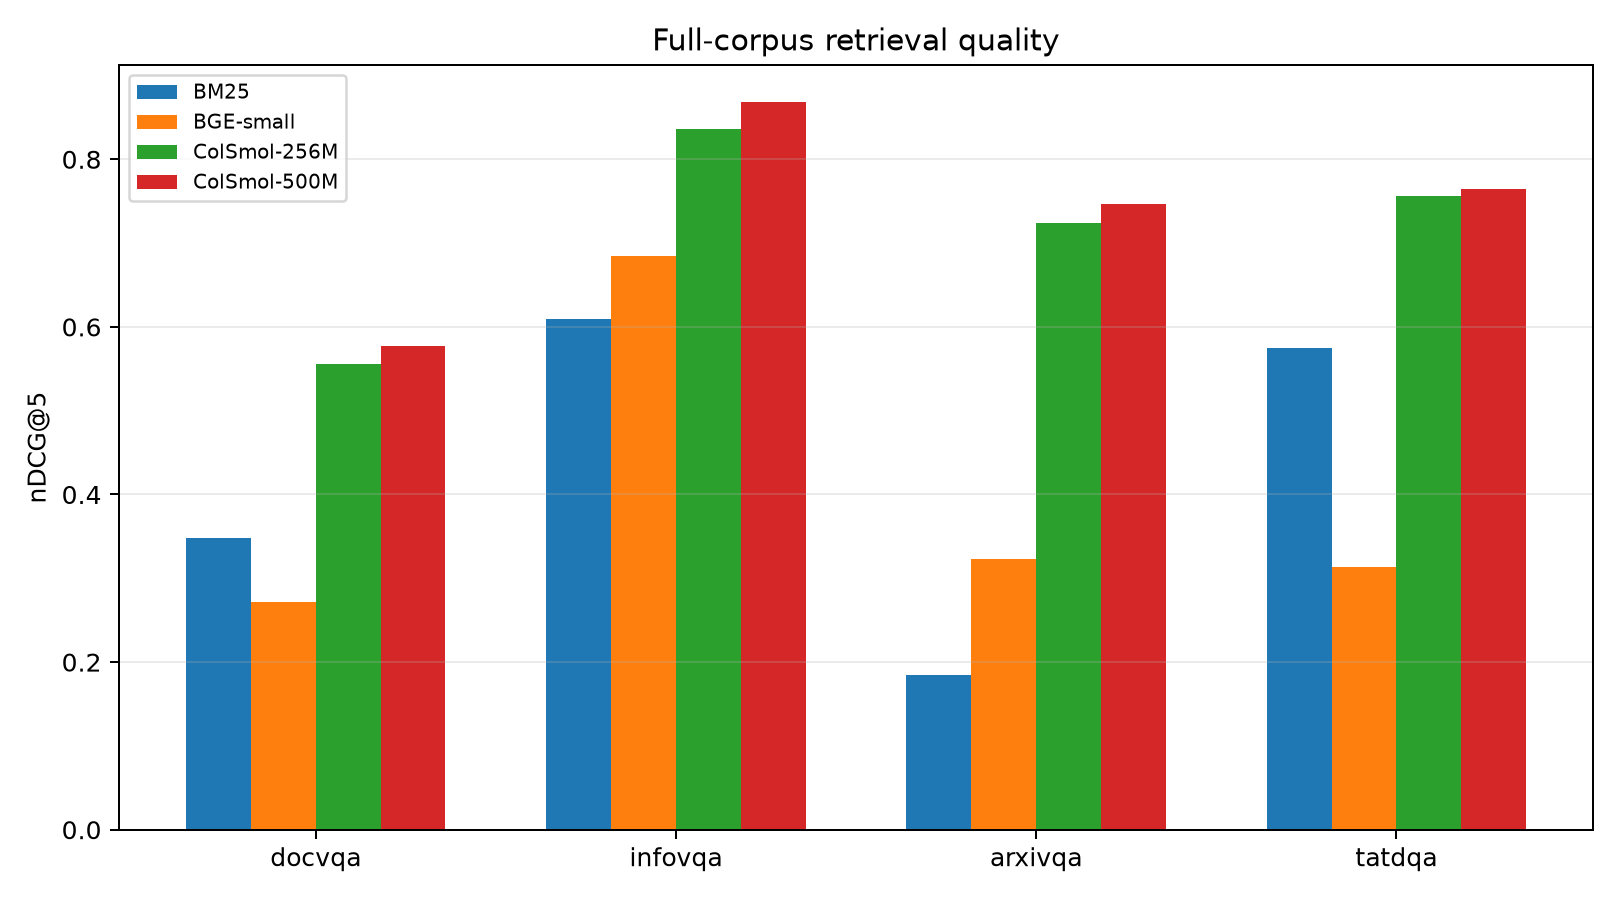
\includegraphics[width=0.62\textwidth]{../artifacts/summary/figures/main_ndcg5.png}
\caption{Main nDCG@5 comparison generated from the committed result JSON files.}
\label{fig:main}
\end{figure}

Three observations tell the main story.
\begin{enumerate}
  \item \textbf{Late interaction is the decisive component.} With the same 500M encoder, MaxSim exceeds global pooling by 38.6 points on DocVQA, 31.4 on InfoVQA, 49.4 on ArxivQA, and 48.1 on TatDQA. Local matching is therefore not a cosmetic scoring change; it prevents crucial page regions from being averaged away.
  \item \textbf{Visual retrieval is consistently strongest.} MaxSim-500M beats the best text baseline by 23.0, 18.4, 42.4, and 19.0 points on the four datasets. The largest gap occurs on scientific figures, exactly where OCR has both a representational disadvantage and incomplete text coverage.
  \item \textbf{Scaling helps, but less than representation.} Moving from 256M to 500M improves MaxSim by 2.2, 3.2, 2.2, and 0.8 points. By contrast, changing global pooling to MaxSim gives tens of points. For this scale, keeping local tokens is more important than doubling the checkpoint class.
\end{enumerate}

For the 500M MaxSim system, Recall@1 / Recall@5 / Recall@10 is 50.0/64.3/71.5 on DocVQA, 82.4/90.5/92.7 on InfoVQA, 67.0/81.2/85.8 on ArxivQA, and 64.1/87.4/93.7 on TatDQA. Thus, most remaining errors are not only ordering errors: on DocVQA, 28.5\% of queries still have no relevant page in the top ten.

\subsection{Compression ablation}

\begin{table}[H]
\centering
\caption{Smallest configuration retaining at least 95\% of the uncompressed nDCG@5. All selected configurations use k-means.}
\label{tab:compression}
\begin{tabular}{lrrrrr}
\toprule
Dataset & Tokens kept & Base nDCG & Compressed nDCG & Base MB & Compressed MB \\
\midrule
DocVQA & 25\% & 57.8 & 56.6 & 129.36 & 32.36 \\
InfoVQA & 12.5\% & 86.9 & 83.4 & 87.08 & 10.84 \\
ArxivQA & 12.5\% & 74.7 & 71.8 & 107.02 & 13.35 \\
TatDQA & 25\% & 76.5 & 73.0 & 72.38 & 18.11 \\
\bottomrule
\end{tabular}
\end{table}

Equation~\ref{eq:memory} predicts the almost linear storage reduction visible in Table~\ref{tab:compression}: retaining one eighth of the tokens gives roughly one eighth of the index. K-means is the strongest aggressive compressor because its centroids preserve occupied regions of embedding space. Uniform and random selection may discard rare but decisive tokens; contiguous mean pooling may mix unrelated neighbouring regions.

\begin{figure}[H]
\centering
\begin{minipage}{0.49\textwidth}\centering
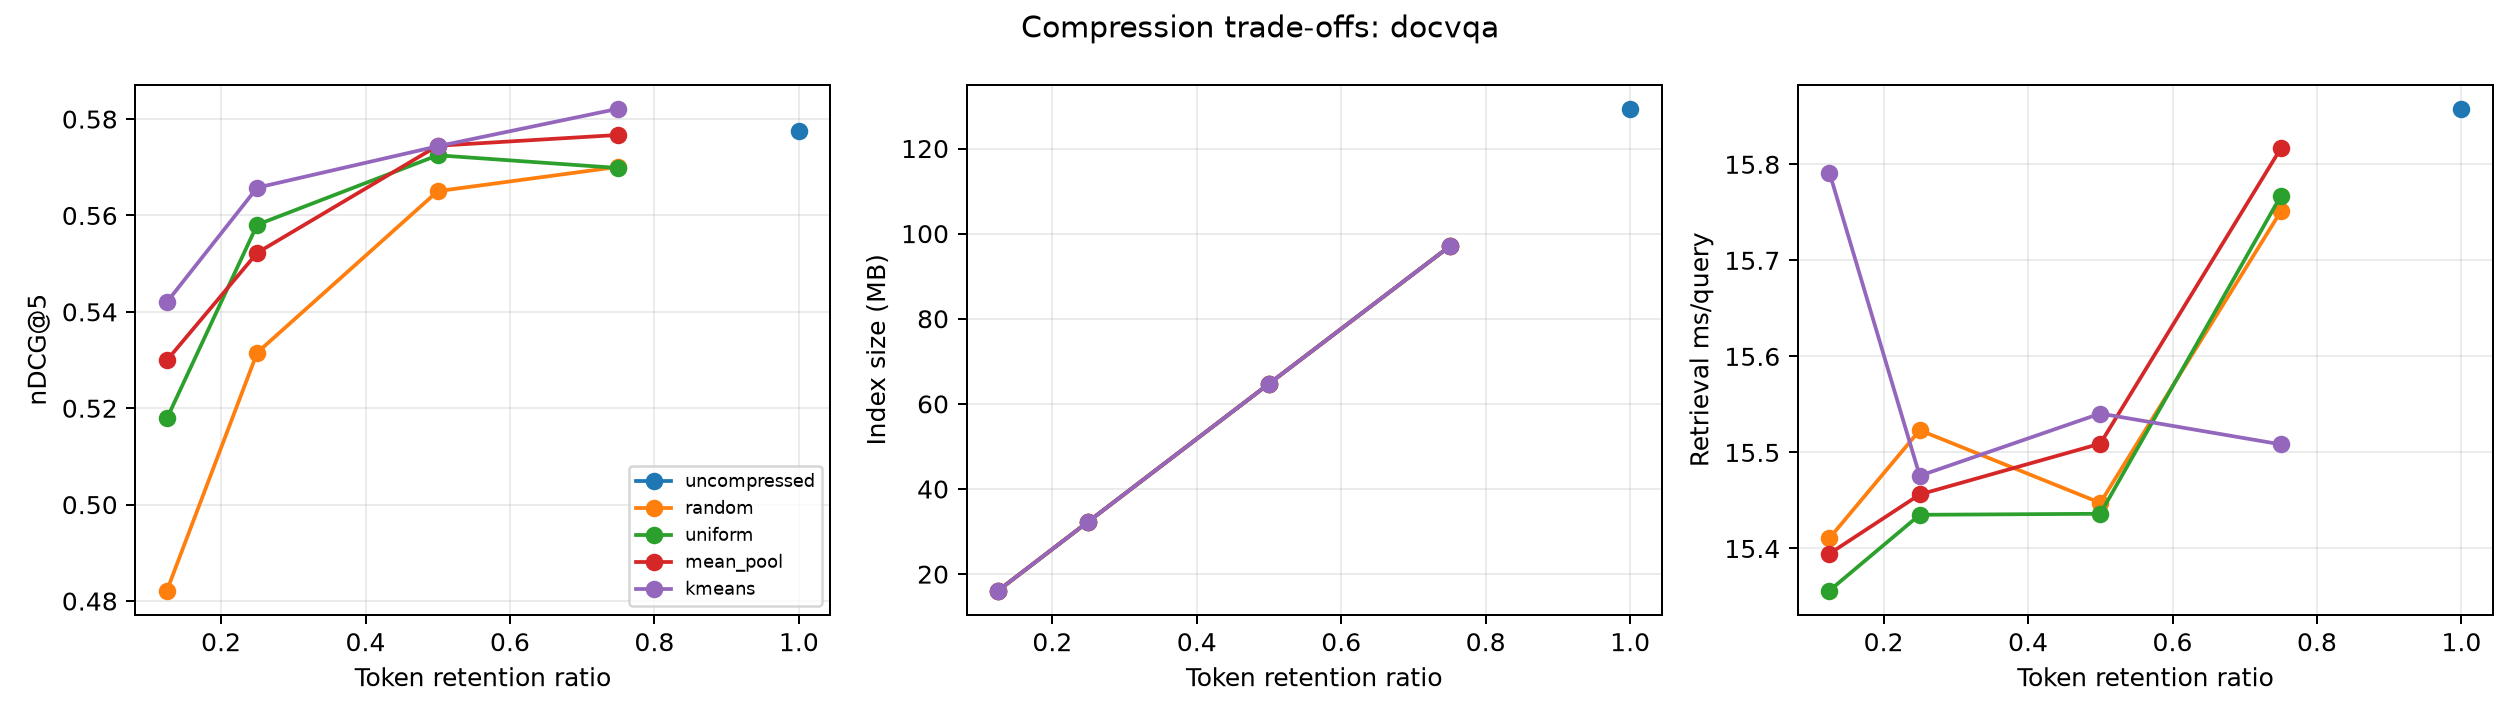
\includegraphics[width=\linewidth]{../artifacts/summary/figures/compression_docvqa.png}
\end{minipage}\hfill
\begin{minipage}{0.49\textwidth}\centering
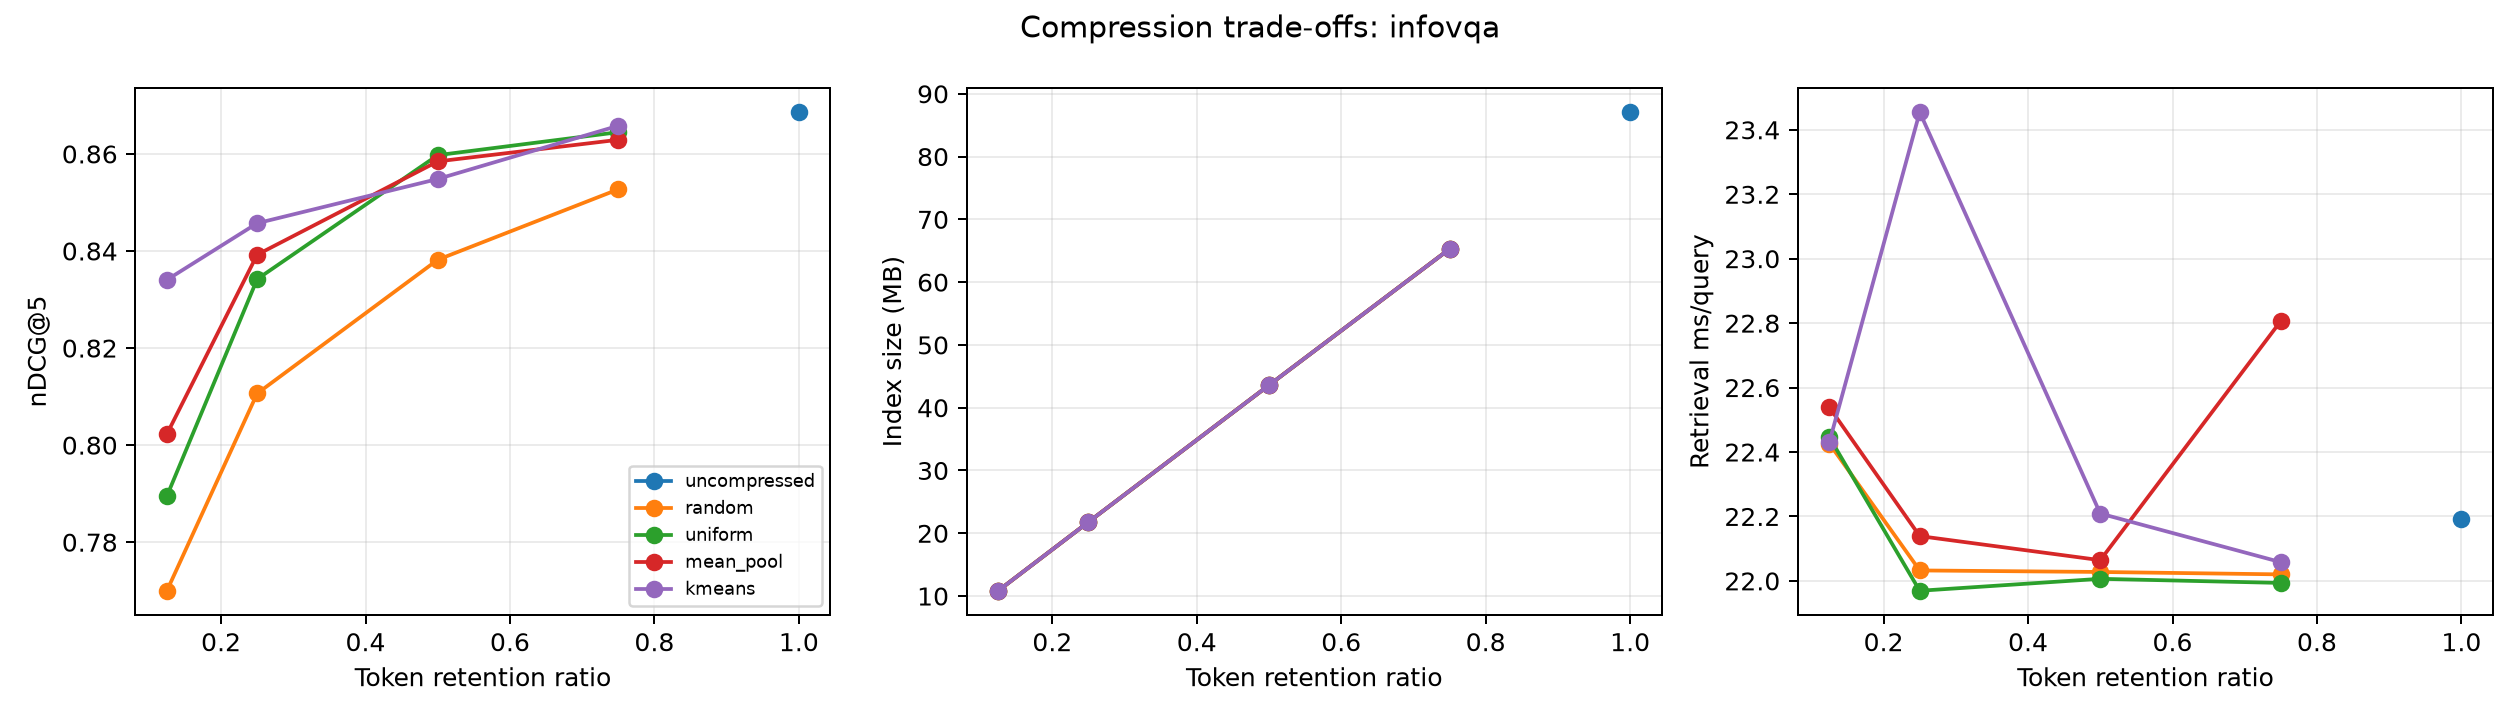
\includegraphics[width=\linewidth]{../artifacts/summary/figures/compression_infovqa.png}
\end{minipage}
\vspace{0.4em}
\begin{minipage}{0.49\textwidth}\centering
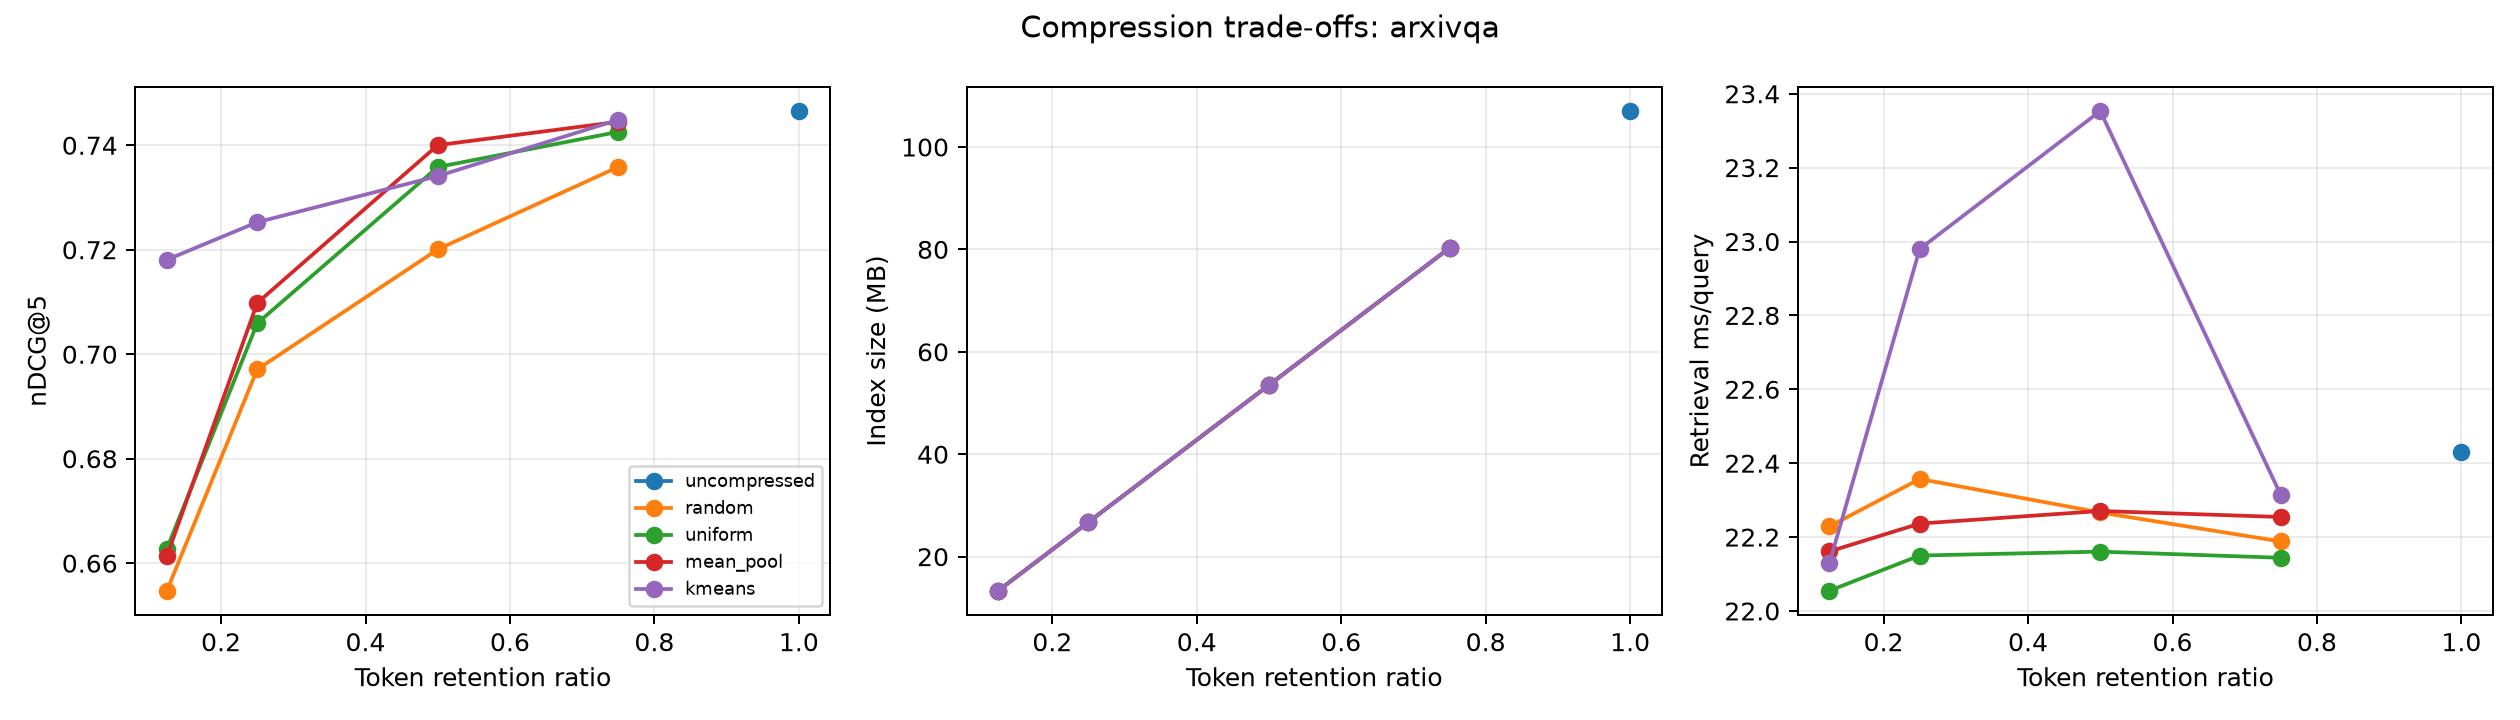
\includegraphics[width=\linewidth]{../artifacts/summary/figures/compression_arxivqa.png}
\end{minipage}\hfill
\begin{minipage}{0.49\textwidth}\centering
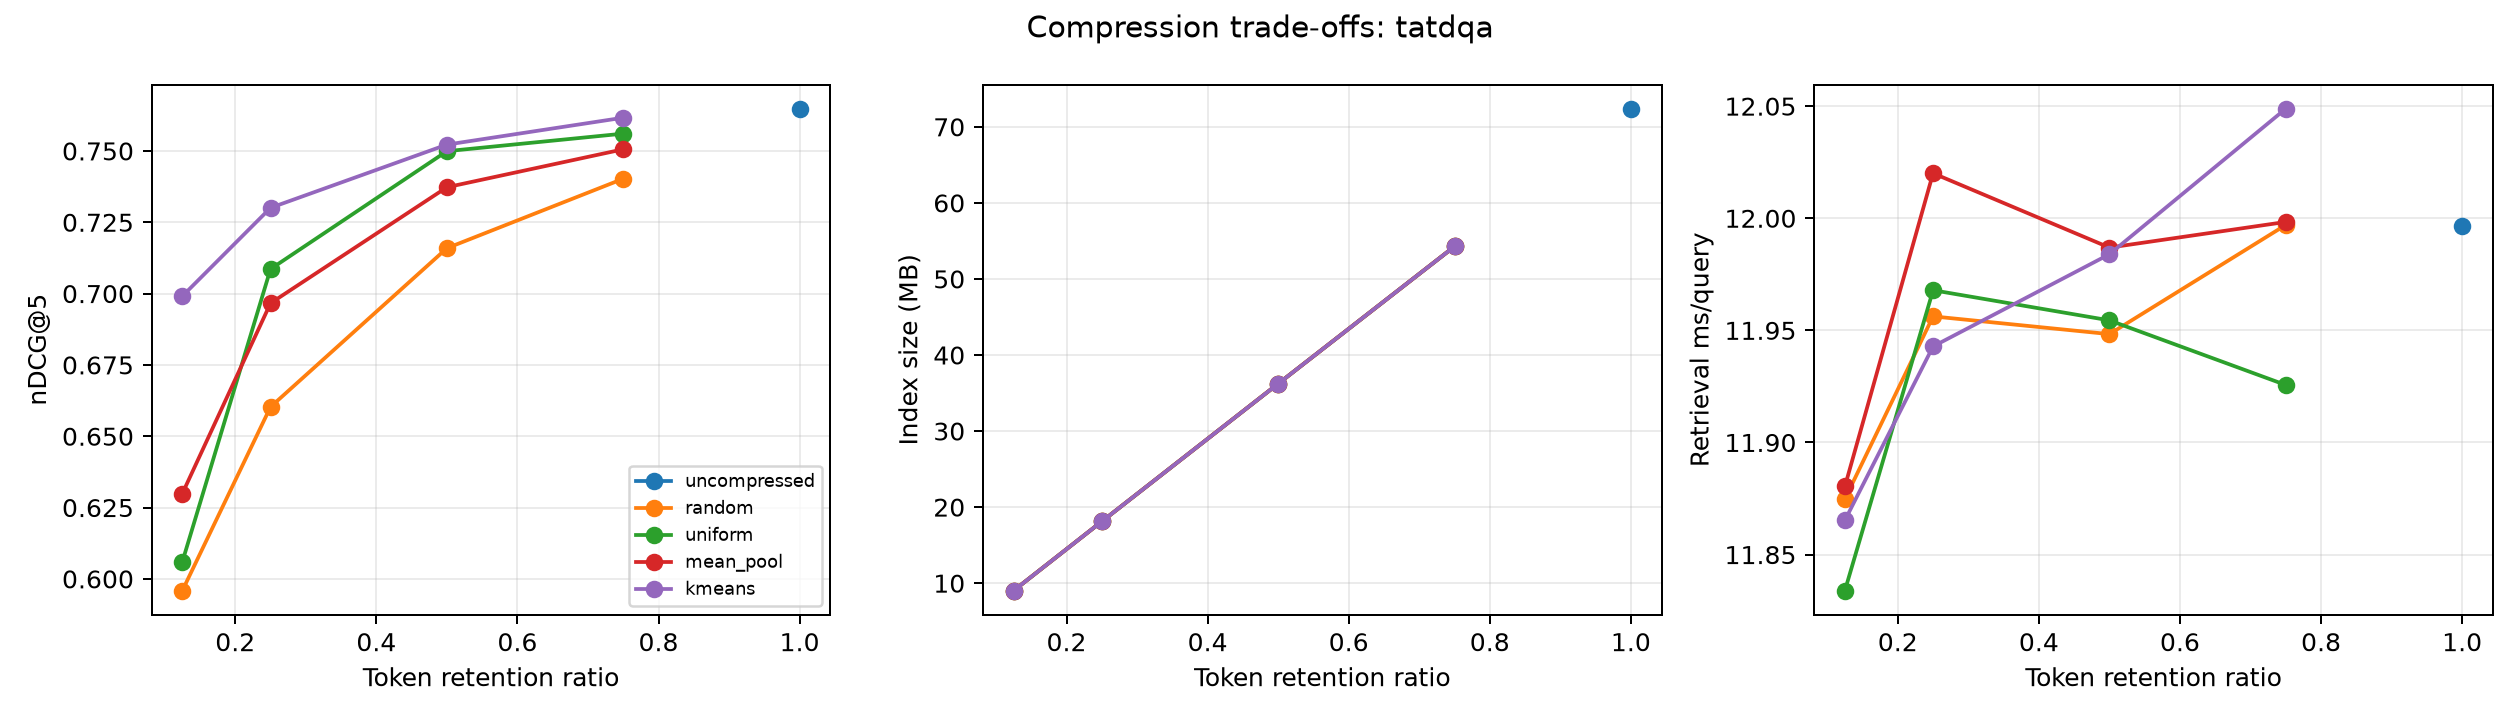
\includegraphics[width=\linewidth]{../artifacts/summary/figures/compression_tatdqa.png}
\end{minipage}
\caption{Quality--storage trade-offs for four compression methods. Random results aggregate three seeds; deterministic methods use one run.}
\label{fig:compression}
\end{figure}

Compression did \emph{not} consistently reduce measured query latency. For example, DocVQA falls from 16.06 to 15.48~ms/query at its chosen point, whereas InfoVQA rises from 16.68 to 22.43~ms/query. At these corpus sizes, GPU launch, batching, padding, top-$k$, and sorting overhead can dominate the number of dot products. The defensible conclusion is therefore strong memory savings with preserved quality, not a universal latency speed-up.

\subsection{Computational requirements}

\begin{table}[H]
\centering
\caption{Measured 500M visual-system efficiency. Encoding peak VRAM is about 2.9~GiB on every dataset.}
\begin{tabular}{lrrrr}
\toprule
Dataset & Page encode (ms) & Query encode (ms) & MaxSim (ms/query) & Index (MB) \\
\midrule
DocVQA & 693.1 & 16.5 & 16.1 & 129.36 \\
InfoVQA & 500.6 & 16.4 & 16.7 & 87.08 \\
ArxivQA & 577.7 & 21.2 & 22.7 & 107.02 \\
TatDQA & 706.2 & 16.5 & 9.1 & 72.38 \\
\bottomrule
\end{tabular}
\end{table}

Page encoding is the expensive offline operation; query encoding and scoring are online. The index remains small here because the benchmark corpora contain only 277--500 pages. For a million pages with 1,000 tokens/page, $d=128$, and FP16 storage, Equation~\ref{eq:memory} gives approximately 238~GiB, which motivates compression or specialised multi-vector indexing for deployment.

\section{Qualitative analysis: where the numbers come from}

Table~\ref{tab:cases} traces individual questions through the rankings. These are not generated explanations of page content; they are direct case studies from the stored per-query ranks.

\begin{table}[H]
\centering
\caption{Representative retrieval cases. Lower rank is better.}
\label{tab:cases}
\small
\begin{tabularx}{\textwidth}{lYrrrr}
\toprule
Dataset & Query & MaxSim & Global & BM25 & BGE \\
\midrule
ArxivQA & What can be inferred about the term ``alexa'' in the given figure? & \best{1} & 234 & 400 & 478 \\
InfoVQA & What does ``R'' stand for? & \best{1} & 239 & 293 & 430 \\
TatDQA & What was the percentage change in the net total between 2018 and 2019? & \best{1} & 243 & 137 & 177 \\
InfoVQA & Which is element 67 on the periodic table? & 44 & 23 & \best{1} & \best{1} \\
DocVQA & What are the letters in the monogram logo at the top right? & 447 & 497 & 45 & 339 \\
ArxivQA & What does the figure primarily illustrate? & 385 & 286 & 480 & \best{4} \\
\bottomrule
\end{tabularx}
\end{table}

The first three cases show the advantage of local visual evidence. A term inside a plot, a one-letter infographic label, or a relationship spanning table cells can be matched without requiring OCR to linearise the whole page. The periodic-table case shows the opposite: a distinctive fact expressed cleanly in text is ideal for lexical or dense text retrieval.

The failures are equally informative. A tiny monogram in a named corner requires both fine visual resolution and explicit spatial grounding; neither representation reliably solves it. The generic question ``What does the figure primarily illustrate?'' contains few discriminative words, so many scientific pages can look semantically plausible. BGE ranks the relevant page fourth, demonstrating that visual and text channels make complementary errors rather than forming a strict hierarchy.

\section{Discussion, limitations, and threats to validity}

\paragraph{What was learned.} The strongest conclusion is architectural: preserving a set of local descriptors and delaying interaction until the query arrives is dramatically more effective than compressing a page to one vector. The 500M model is the best tested system, but the 256M MaxSim model already beats every text and global baseline. K-means then recovers much of the storage cost without erasing the advantage.

\paragraph{OCR comparability.} Text baselines depend on supplied Tesseract artifacts. Non-empty OCR coverage is 84.4\% on ArxivQA, while the visual methods see all 500 page images. This is a real operational advantage of the visual route, but it also means that the ArxivQA gap cannot be attributed purely to representation quality. The other three datasets have 99.2--100\% non-empty OCR coverage.

\paragraph{Scale.} Full benchmark splits were used, but each retrieval corpus is small. Brute-force GPU MaxSim is reasonable for 277--500 pages and does not prove million-page scalability. Approximate multi-vector search, sharding, candidate generation, or reranking would be necessary at production scale.

\paragraph{No task-specific training.} This is an evaluation and ablation project. It uses released ColSmol checkpoints and does not fine-tune on the four test sets. That choice gives a clean study of off-the-shelf representations, but does not answer how contrastive fine-tuning or parameter-efficient adaptation would change the trade-off.

\paragraph{No answer-generation evaluation.} Although RAG motivates the work, the experiments stop after retrieval. There is no language-model answer, faithfulness metric, or hallucination study. Calling the current system a complete RAG pipeline would therefore be incorrect. The honest claim is that it implements and evaluates the retriever required by a future visual RAG system.

\paragraph{Qualitative evidence.} Per-query successes and failures are analysed, satisfying the need for qualitative interpretation, but no token-to-region heatmaps were generated. Future work should overlay each query token's argmax location from Equation~\ref{eq:maxsim} on the page. This would turn the ranking score into a spatial explanation and help distinguish encoder failures from ambiguous annotations.

\section{From this retriever to a complete RAG system}

The next engineering step is short, but its evaluation is a separate experiment:
\begin{enumerate}
  \item index each page once with compressed ColSmol vectors;
  \item retrieve the top-$K$ page images with MaxSim;
  \item give those images and the question to a vision-language generator;
  \item require citations to page identifiers;
  \item score retrieval and generation separately, including answer correctness and faithfulness.
\end{enumerate}
This separation is important. Retrieval Recall@$K$ asks whether the evidence was available; answer accuracy asks whether the generator used it; faithfulness asks whether the answer is actually supported. Conflating the three makes a failure impossible to diagnose.

\section{Conclusion}

This project began with a simple fact: generation cannot use evidence that retrieval fails to find. For visually rich documents, OCR-first text retrieval discards part of the signal before matching begins. ColSmolVLM instead represents a page as many local visual vectors, and MaxSim lets each query concept find its strongest region. On four complete ViDoRe tasks, that design beats BM25, dense OCR-text retrieval, and global visual pooling. The largest gain comes not from model size but from retaining local structure. K-means compression then keeps at least 95\% of baseline nDCG@5 with only one eighth to one quarter of the visual tokens. The resulting system is a lightweight, reproducible, and mathematically interpretable retriever---a strong foundation for multimodal RAG, while remaining explicit about what has not yet been generated or evaluated.

\section*{Implementation provenance and academic integrity}
The ColSmolVLM checkpoints, ColPali/ColBERT concepts, BGE checkpoint, MTEB/ViDoRe datasets, and Tesseract OCR artifacts are prior work and are cited below. The project contribution is the reproducible evaluation implementation, verified OCR-to-corpus join, global-pooling ablation, 256M/500M comparison, token-compression study, efficiency measurement, aggregation, plots, and per-query failure analysis. No benchmark result is presented as model training performed in this project.

\begin{thebibliography}{9}
\bibitem{lewis2020rag} P. Lewis et al., ``Retrieval-Augmented Generation for Knowledge-Intensive NLP Tasks,'' \emph{NeurIPS}, 2020. \url{https://arxiv.org/abs/2005.11401}
\bibitem{robertson2009bm25} S. Robertson and H. Zaragoza, ``The Probabilistic Relevance Framework: BM25 and Beyond,'' \emph{Foundations and Trends in Information Retrieval}, 3(4), 2009. \url{https://doi.org/10.1561/1500000019}
\bibitem{xiao2023cpack} S. Xiao et al., ``C-Pack: Packaged Resources To Advance General Chinese Embedding,'' 2023. \url{https://arxiv.org/abs/2309.07597}
\bibitem{khattab2020colbert} O. Khattab and M. Zaharia, ``ColBERT: Efficient and Effective Passage Search via Contextualized Late Interaction over BERT,'' \emph{SIGIR}, 2020. \url{https://doi.org/10.1145/3397271.3401075}
\bibitem{faysse2024colpali} M. Faysse et al., ``ColPali: Efficient Document Retrieval with Vision Language Models,'' \emph{ICLR}, 2025. \url{https://arxiv.org/abs/2407.01449}
\bibitem{colsmolmodel} ViDoRe, ``colSmol-500M Model Card.'' \url{https://huggingface.co/vidore/colSmol-500M}
\bibitem{smolvlm2025} A. Marafioti et al., ``SmolVLM Grows Smaller---Introducing the 256M \& 500M Models,'' Hugging Face, 2025. \url{https://huggingface.co/blog/smolervlm}
\bibitem{vidoredata} ViDoRe, ``Visual Document Retrieval Benchmark Collection.'' \url{https://huggingface.co/collections/vidore/vidore-benchmark}
\end{thebibliography}

\appendix
\section{Artifact map}

The report can be audited from repository artifacts rather than reconstructed from prose:
\begin{itemize}
  \item \code{artifacts/results/visual/}: eight full visual evaluations;
  \item \code{artifacts/results/text/}: four OCR text-baseline evaluations;
  \item \code{artifacts/results/compression/}: 100 compression configurations and manifests;
  \item \code{artifacts/summary/main\_results.csv}: 24 primary method--dataset rows;
  \item \code{artifacts/summary/compression\_aggregate.csv}: 68 aggregated compression rows;
  \item \code{artifacts/summary/failure\_analysis.csv}: 30 difficult queries;
  \item \code{artifacts/results/environment\_diagnostic.json}: software and GPU provenance.
\end{itemize}

\section{Minimal reproduction command}

The repository README documents every experiment individually. The complete tested pipeline is:
\begin{lstlisting}[language=bash]
source rag/bin/activate
GPU_ID=2 bash scripts/run_all_experiments.sh
\end{lstlisting}

\end{document}
